%% LyX 2.3.3 created this file.  For more info, see http://www.lyx.org/.
%% Do not edit unless you really know what you are doing.
\documentclass{IJFV}
\usepackage[T1]{fontenc}
\usepackage[utf8]{inputenc}
\usepackage{geometry}
\geometry{verbose}
\setlength{\parskip}{\smallskipamount}
\setlength{\parindent}{0pt}
\synctex=-1
\usepackage{color}
%\usepackage{babel}
\usepackage{array}
\usepackage{float}
\usepackage{url}
\usepackage{algorithm2e}
%\usepackage{amsbsy}
%\usepackage{amstext}
%\usepackage{amsthm}
%\usepackage{amssymb}
\usepackage{graphicx}
\usepackage[unicode=true]
 {hyperref}

\makeatletter

%%%%%%%%%%%%%%%%%%%%%%%%%%%%%% LyX specific LaTeX commands.
%% Because html converters don't know tabularnewline
\providecommand{\tabularnewline}{\\}

%%%%%%%%%%%%%%%%%%%%%%%%%%%%%% Textclass specific LaTeX commands.
\numberwithin{equation}{section}
\numberwithin{figure}{section}
\theoremstyle{plain}
\newtheorem{thm}{\protect\theoremname}
\theoremstyle{remark}
\newtheorem{rem}[thm]{\protect\remarkname}

%%%%%%%%%%%%%%%%%%%%%%%%%%%%%% User specified LaTeX commands.
\usepackage{tikz}
\usepackage{tikz-3dplot}
\usetikzlibrary{patterns}
\usetikzlibrary{matrix}
\usetikzlibrary{decorations.pathmorphing}
\usetikzlibrary{decorations.pathreplacing}
\usetikzlibrary{decorations.markings}
\usetikzlibrary{decorations.shapes}
\usetikzlibrary{arrows}
\usepackage{pgfplots}
\pgfplotsset{compat=newest}


\usepackage{babel}

\newcommand{\inmod}{\color{black}}
\newcommand{\outmod}{\color{black}}

\RestyleAlgo{ruled}
\LinesNumbered

\makeatother

\providecommand{\remarkname}{Remark}
\providecommand{\theoremname}{Theorem}

\begin{document}
\IJFVtitle{DG solver with StarPU}{Optimization of a discontinuous Galerkin solver with OpenCL and StarPU}
\IJFVauthor{Bérenger Bramas$^\dagger$} 
\IJFVinstitution{$^\dagger$Université de Strasbourg, Icube, Inria Camus.}
\IJFVemail{berenger.bramas@inria.fr}
\IJFVauthor{Philippe Helluy, Laura Mendoza$^\star$} 
\IJFVinstitution{$^\star$Université de Strasbourg, IRMA, Inria Tonus.}
\IJFVemail{philippe.helluy@unistra.fr, laura.mendoza@inria.fr}
\IJFVauthor{Bruno Weber$^\ddagger$} 
\IJFVinstitution{$^\ddagger$AxesSim, Illkirch. }
\IJFVemail{bruno.weber@axessim.fr}
\IJFVabstract{\inmod Since the recent advance in microprocessor design, the optimization
	of computing software becomes more and more technical. One of the
	difficulties is to transform sequential algorithms into parallel ones.
	A possible solution is the task-based design. In this approach, it is  possible
	to describe the parallelization possibilities of the algorithm automatically.
	The task-based design is also a good strategy to optimize software
	in an incremental way. The objective of this paper is to describe
	a practical experience of a task-based parallelization of a Discontinuous
	Galerkin method in the context of electromagnetic simulations. 
     The task-based description is managed by the StarPU runtime. Additional acceleration
     is obtained by OpenCL. 
}
\IJFVkeywords{Discontinuous Galerkin, StarPU, OpenCL, hybrid parallelism.}



%\maketitle

\section{Introduction}
\let\thefootnote\relax\footnotetext{This work has obtained support from the ANR EXAMAG project and the
	BPI France HOROCH project.} 
The development of engineering simulation software faces two major
antagonist issues. On the one hand, the user is interested in handling
more and more complex physical phenomena, in devices with arbitrary
geometries. These constraints require to adopt a generic and abstract
software engineering approach in order to ensure the generality of
the code. On the other hand, the user also wants to harness the full
computational power of his hybrid computer. This requirement generally
imposes to use low-level hardware optimization hacks that are not
always compatible with a generic and universal approach. In addition,
as the hardware evolves, optimizations of yesterday are not necessarily
relevant for the devices of tomorrow.

\inmod The Discontinuous Galerkin algorithm is a general method for
approximating system of conservation laws coming from physics. For
a recent review of this method, we refer to \cite{hesthaven2007nodal}.
This method is well adapted to parallel computing, GPU computing and
various software optimization. See for instance \cite{klockner2013high,helluy2016asynchronous}.
However these optimizations are complicated to program with low-level
librairies. The task is even more complex when the software is run
on a hybrid computer made of different computing accelerators. The
aim of this work is to describe a practical optimization of the Discontinuous
Galerkin method that tries to keep the software design as simple as
possible.\outmod 

\inmod Several software environments have been developed recently
for addressing massively multicore accelerators, such as Graphic Processing
Units (GPUs). CUDA is one of these tools, it is devoted to NVIDIA
GPUs. OpenCL (Open Computing Language) is another tool. Its main advantage
over CUDA is that it can be used with hardware of different brands
(NVIDIA, AMD, Intel, ARM, \textit{etc.}). OpenCL is a nice software
environment for optimization purposes. OpenCL specifies programming
languages (based on C99 and C++11) for programming these devices and
application programming interfaces (APIs) to control the platform
and execute programs on the compute devices. OpenCL provides a standard
interface for parallel computing
%\footnote{\href{https://en.wikipedia.org/wiki/OpenCL}{https://en.wikipedia.org/wiki/OpenCL}}.
OpenCL has been used successfully in several works for accelerating
Finite Volume (FV) or Discontinuous Galerkin (DG) programs. See for
instance \cite{crestetto2012resolution,klockner2013high,helluy2014multi,strub:tel-01651258,helluy2016asynchronous,essadki2018task}\outmod .
It presents the good balance between an abstract view of the computing
devices and some important hardware aspects, such as local memory
for accelerating data transfers or subgroups for minimizing synchronization
barriers. However depending on architecture, optimizations written
for one accelerator may be completely irrelevant for another one.
A CPU (Central Processing Unit), a discrete GPU (Graphic Processing
Unit) or an IGP (Integrated Graphic Processor) have completely different
behavior concerning local cache memory optimizations. For instance,
cache prefetching is generally efficient for discrete GPUs while inefficient
for IGPs.

In this paper, we present our practical approach to this issue, with
the help of the StarPU runtime system. StarPU is developed at Inria
Bordeaux since 2006. StarPU is a runtime C library based on the dataflow
paradigm. The programmer has to split the computation workload into
abstract computational tasks. Each task processes data buffers that
can be in \texttt{read} (R), \texttt{write} (W) or \texttt{read/write}
(RW) mode.

The tasks are then conveniently implemented into  \emph{codelets}.
It is possible (and recommended) to write several implementations
of the same task into several codelets. For instance, one can imagine
writing a standard codelet in C for validation purposes and one or
several optimized OpenCL codelets. The user then submits the tasks
in a sequential way to StarPU. At runtime, StarPU is able to construct
a task graph based on buffer dependencies. The tasks are submitted
to the available accelerators, in parallel if the dependencies allow
it. StarPU decides at runtime which version of the codelet (C or OpenCL)
is executed. \textcolor{black}{The scheduler is in charge of the distribution
of the tasks over the processing units. Dozens of schedulers are provided
by StarPU and it is possible to create a custom scheduler to plug
it inside StarPU. Some schedulers take into account data locality
or use performance models }by measuring the efficiency of the different
codelets' implementations in order to choose the best one\textcolor{black}{.}
In addition, StarPU automatically handles data transfers between the
accelerators\textcolor{black}{: when a task is assigned to a processing
unit, StarPU moves the data that are not already on the processing
unit's memory and it can also evict old data if the available space
is not enough.}

With StarPU, implementing a complex dataflow of OpenCL kernels becomes
easier. Indeed, the programmer does not have to handle the kernel
dependencies with OpenCL events. In addition, it is possible to first
write a well validated pure C version of the software, with only C
codelets. Then, one can enrich the tasks with OpenCL codelets, which
allows an incremental optimization of the code. At each stage, StarPU
should be able to use the available codelets in an efficient way.

In this paper, we describe how we applied the StarPU philosophy in
order to optimize a discontinuous finite element solver for conservation
laws. \inmod  A similar experience is also presented for instance
in \cite{essadki2018task}\outmod . The outlines are as follows:
first we will present in its main lines the Discontinuous Galerkin
(DG) scheme that is used in the solver. Then, after a short presentation
of StarPU, we will explain how we have integrated the OpenCL optimizations
into the DG solver. Finally, we will present some numerical experiments.

\section{Discontinuous Galerkin method}

\global\long\def\vf{\mathbf{{f}}}%
 
\global\long\def\vg{\mathbf{{g}}}%
 
\global\long\def\vh{\mathbf{{h}}}%
 
\global\long\def\vs{\mathbf{{s}}}%
 
\global\long\def\vV{\mathbf{V}}%
 
\global\long\def\vx{\mathbf{x}}%
 
\global\long\def\v#1{\mathbf{#1}}%
 
\global\long\def\vq{\mathbf{q}}%
 
\global\long\def\vw{\mathbf{w}}%
 
\global\long\def\ddim{D}%
 
\global\long\def\dorder{d}%
 
\global\long\def\normal{\mathbf{n}}%
 
\global\long\def\flux{\mathbf{q}}%
 
\global\long\def\Vu{\mathbf{u}}%
 
\global\long\def\Vvi{\mathbf{v}_{i}}%

The Discontinuous Galerkin (DG) method is a general finite element
method for approximating systems of conservation laws of the form
\[
\partial_{t}\v w+\sum_{k=1}^{\ddim}\partial_{k}\v f^{k}(\v w)=0.
\]
The unknown is the vector of conservative variables $\v w(\v x,t)\in\mathbb{R}^{m}$
depending on the space variable $\v x=(x^{1},\ldots,x^{\ddim})\in\mathbb{R}^{\ddim}$
and on time $t$. In this paper, the space dimension is $\ddim=3$.
\inmod The flux components $\v f^{k}$, $k=1\ldots D$, are smooth
functions from $\mathbb{R}^{m}$ to $\mathbb{R}^{m}$.\outmod  We
adopt the notations $\partial_{t}$ for the partial derivative with
respect to $t$ and $\partial_{k}$ for the partial derivative with
respect to $x^{k}$. Let $\v n=(n_{1},\ldots,n_{\ddim})\in\mathbb{R}^{\ddim}$
be a spatial direction. \inmod The flux $\v f$ is a smooth function
from $\mathbb{R}^{m}\times\mathbb{R}^{D}$ to $\mathbb{R}^{m}$,\outmod 
defined by 
\[
\v f(\v w,\v n)=\sum_{k=1}^{\ddim}n_{k}\v f^{k}(\v w).
\]
For instance, in this work we consider the numerical simulation of
an electromagnetic wave. In this particular case, the conservative
variables are 
\[
\v w=(\v E^{\mathrm{T}},\v H^{\mathrm{T}},\lambda,\mu)^{\mathrm{T}}\in\mathbb{R}^{m},\quad m=8,
\]
where $\v E\in\mathbb{R}^{3}$ is the electric field, $\v H\in\mathbb{R}^{3}$
is the magnetic field and $\lambda$, $\mu$ are divergence cleaning
potentials (\cite{munz2000divergence}). The flux is given by 
\[
\v f(\v w,\v n)=\left(\begin{array}{c}
-\v n\times\v H+\lambda\v n\\
\v n\times\v E+\mu\v n\\
c\v n\cdot\v E\\
c\v{n\cdot H}
\end{array}\right)
\]
and $c>1$ is the divergence cleaning parameter.

\inmod The computational domain $\Omega$ is an open set of $\mathbb{R}^{D}$.\outmod 
We consider a mesh $\mathcal{M}$ of $\Omega$ made of $N_{c}$ open
sets, called \emph{cells}, $\mathcal{M}=\left\{ L_{i},\,i=1\ldots N_{c}\right\} $.
In the most general setting, the cells satisfy 
\begin{enumerate}
\item $L_{i}\cap L_{j}=\emptyset$, if $i\neq j$; 
\item $\overline{\cup_{i}L_{i}}=\overline{\Omega}.$ 
\end{enumerate}
In each cell $L\in\mathcal{M}$, we consider a basis of \inmod $N_{d}$
functions $(\varphi_{L,i}(\vx))_{i=0\ldots N_{\dorder}-1}$. The basis
functions are constructed by tensor products of polynomials of order
$\dorder$. Therefore $N_{d}=(d+1)^{D}$\outmod . We denote by $h$
the maximal diameter of the cells. \inmod We assume that the local
approximation $\vw_{L}$ of $\vw$ in cell $L$ is given by 
\[
\vw_{L}(\vx,t)=\sum_{j=0}^{N_{\dorder}-1}\vw_{L,j}(t)\varphi_{L,j}(\vx),\quad\vx\in L.
\]
\outmod The DG formulation then reads: find $\vw_{L,j}$ such that
for all cell $L$ and all test function $\varphi_{L,i}$ 
\begin{equation}
\int_{L}\partial_{t}\vw_{L}\varphi_{L,i}-\int_{L}\vf(\vw_{L},\boldsymbol{\nabla}\varphi_{L,i})+\int_{\partial L}\vf(\vw_{L},\vw_{R},\v n)\varphi_{L,i}=0.\label{eq:dg_var}
\end{equation}
In this formula (see Figure \ref{fig:cell_convention}): 
\begin{itemize}
\item $R$ denotes the neighboring cell to $L$ along its boundary $\partial L\cap\partial R$,
or the exterior of $\Omega$ on $\partial L\cap\partial\Omega$. 
\item $\normal=\normal_{LR}$ is the unit normal vector on $\partial L$
oriented from $L$ to $R$. 
\item $\vw_{R}$ denotes the value of $\vw$ in the neighboring cell $R$
on $\partial L\cap\partial R$. 
\item If $L$ is a boundary cell, one may have to use the boundary values
instead: $\vw_{R}=\vw_{b}$ on $\partial L\cap\partial\Omega$. 
\item $\vf(\vw_{L},\vw_{R},\v n)$ is the standard upwind numerical flux
encountered in many finite volume or DG methods. 
\end{itemize}
\begin{figure}
\begin{centering}
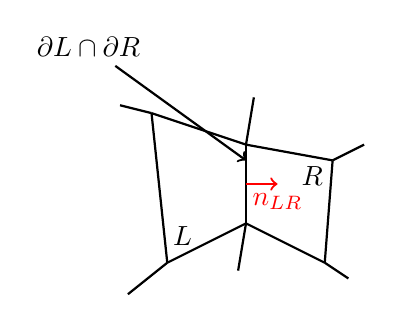
\begin{tikzpicture}[scale=1]
% intersection 
\draw[thick] (0,1) -- (0,0); \draw[->, thick, color=red] (0,0.5) -- (0.4,0.5); \node[below, color=red] at (0.4,0.5) {$n_{LR}$}; \node[above] (n1) at (-2,2) {$\partial L\cap\partial R$}; \draw[->, thick] (n1) -- (0,0.8);
% left  
\draw[thick] (-1,-0.5) -- (0,0); \draw[thick] (-1.2,1.4) -- (0,1); \draw[thick] (-1.2,1.4) -- (-1,-0.5); \node[above right] at (-1.05,-0.4) {$L$}; 
% right  
\draw[thick] (1,-0.5) -- (0,0); \draw[thick] (1.1,0.8) -- (0,1); \draw[thick] (1.1,0.8) -- (1,-0.5); \node[below left] at (1.1,0.85) {$R$};
% other quadrangles
\draw[thick] (0,0) -- (-0.1,-0.6); \draw[thick] (0,1) -- (0.1,1.6); \draw[thick] (-1,-0.5) -- (-1.5,-0.9); \draw[thick] (-1.2,1.4) -- (-1.6,1.5); \draw[thick] (1,-0.5) -- (1.3,-0.7); \draw[thick] (1.1,0.8) -- (1.5,1);  \end{tikzpicture} 
\par\end{centering}
\caption{\label{fig:cell_convention}Convention for the $L$ and $R$ cells
orientation.}
\end{figure}

In our application, we consider hexahedral cells. We have a reference
cell 
\[
\hat{L}=]-1,1[^{\ddim}
\]
\global\long\def\jacob{\boldsymbol{\tau}}%
 and a smooth transformation $\vx=\jacob_{L}(\hat{\vx})$, $\hat{\vx}\in\hat{L}$,
that maps $\hat{L}$ on $L$ 
\[
\jacob_{L}(\hat{L})=L.
\]
We assume that $\jacob_{L}$ is invertible and we denote by $\jacob_{L}'$
its (invertible) Jacobian matrix. We also assume that $\jacob_{L}$
is a direct transformation 
\[
\det\jacob_{L}'>0.
\]
In our implementation, $\jacob_{L}$ is a quadratic map based on hexahedral
curved ``H20'' finite elements with 20 nodes. The mesh of H20 finite
elements is generated by \texttt{gmsh} (\cite{geuzaine2009gmsh}).

On the reference cell, we consider the Gauss-Lobatto points $(\hat{\vx}_{i})_{i=0\ldots N_{\dorder}-1}$,
$N_{\dorder}=(\dorder+1)^{\ddim}$ and associated weights $(\hat{\omega}_{i})_{i=0\ldots N_{\dorder}-1}$.
They are obtained by tensor products of the $(\dorder+1)$ one-dimensional
Gauss-Lobatto (GL) points on $]-1,1[$. The reference GL points and
weights are then mapped to the physical GL points of cell $L$ by
\begin{equation}
\vx_{L,i}=\jacob_{L}(\hat{\vx}_{i}),\quad\omega_{L,i}=\hat{\omega}_{i}\det\jacob_{L}'(\hat{\vx}_{i})>0.\label{eq:map_GL}
\end{equation}
In addition, the six faces of the reference hexahedral cell are denoted
by $F_{\epsilon}$, $\epsilon=1\ldots6$ and the corresponding outward
normal vectors are denoted by $\hat{\normal}_{\epsilon}$. One advantage
of choosing the GL points is that the cells and the faces share the
same quadrature points. We use the following notations to define the
face quadrature weights: 
\begin{itemize}
\item if a GL point $\hat{\vx}_{i}\in F_{\epsilon}$, we denote by $\mu_{i}^{\epsilon}$
the corresponding quadrature weight on face $F_{\epsilon}$;
\item we also use the convention that $\mu_{i}^{\epsilon}=0$ if $\hat{\vx}_{i}$
does not belong to face $F_{\epsilon}$. 
\end{itemize}
Let us remark that a given GL point $\hat{\vx}_{i}$ can belong to
several faces when it is on an edge or in a corner of $\hat{L}$.
Because of symmetry, we observe that if $\mu_{i}^{\epsilon}\neq0$,
then the weight $\mu_{i}^{\epsilon}$ does not depend on $\epsilon$.

We then consider basis functions $\hat{\varphi_{i}}$ on the reference
cell: they are the Lagrange polynomials associated to the Gauss-Lobatto
points and thus satisfy the interpolation property 
\[
\hat{\varphi}_{i}(\hat{\vx}_{j})=\delta_{ij}.
\]
The basis functions on cell $L$ are then defined according to the
formula 
\[
\varphi_{L,i}(\vx)=\hat{\varphi}_{i}(\jacob_{L}^{-1}(\vx)).
\]
In this way, they also satisfy the interpolation property 
\begin{equation}
\varphi_{L,i}(\vx_{L,j})=\delta_{ij}.\label{eq:interp_property}
\end{equation}
In this paper, we only consider conformal meshes: the GL points on
cell $L$ are supposed to match the GL points of cell $R$ on their
common face. Dealing with non-matching cells is the object of a forthcoming
work. Let $L$ and $R$ be two neighboring cells. Let $\vx_{L,j}$
be a GL point in cell $L$ that is also on the common face between
$L$ and $R$. In the case of conformal meshes, it is possible to
define the index $j'$ such that 
\[
\vx_{L,j}=\vx_{R,j'}.
\]

Applying a numerical integration to (\ref{eq:dg_var}), using (\ref{eq:map_GL})
and the interpolation property (\ref{eq:interp_property}), we finally
obtain 
\begin{equation}
\partial_{t}\vw_{L,i}\omega_{L,i}-\sum_{j=0}^{N_{\dorder}-1}\vf(\vw_{L,j},\boldsymbol{\nabla}\varphi_{L,i}(\vx_{L,j}))\omega_{L,j}+\sum_{\epsilon=1}^{6}\mu_{i}^{\epsilon}\vf(\vw_{L,i},\vw_{R,i'},\normal_{\epsilon}(\vx_{L,i}))=0.\label{eq:dg_lobatto}
\end{equation}
We have to detail how the gradients and normal vectors are computed
in the above formula. Let $\v A$ be a square matrix. We recall that
the cofactor matrix of $\v A$ is defined by 
\begin{equation}
\text{co}(\v A)=\det(\v A)\left(\v A^{-1}\right)^{\mathrm{T}}.\label{eq:co_mat}
\end{equation}
The gradient of the basis function is computed from the gradients
on the reference cell using (\ref{eq:co_mat}) 
\[
\boldsymbol{\nabla}\varphi_{L,i}(\vx_{L,j})=\frac{1}{\det\jacob_{L}'(\hat{\vx}_{j})}\text{co}(\jacob_{L}'(\hat{\vx}_{j}))\hat{\nabla}\hat{\varphi}_{i}(\hat{\vx}_{j}).
\]
In the same way, the scaled normal vectors $\v n_{\epsilon}$ on the
faces are computed by the formula 
\[
\normal_{\epsilon}(\vx_{L,i})=\text{co}(\jacob_{L}'(\hat{\vx}_{i}))\hat{\normal}_{\epsilon}.
\]
We introduce the following notation for the cofactor matrix
\global\long\def\comat{\mathbf{c}}%
 
\[
\comat_{L,i}=\text{co}(\jacob_{L}'(\hat{\vx}_{i})).
\]
The DG scheme then reads 
\begin{equation}
\partial_{t}\vw_{L,i}-\frac{1}{\omega_{L,i}}\sum_{j=0}^{N_{\dorder}-1}\vf(\vw_{L,j},\comat_{L,j}\hat{\nabla}\hat{\varphi}_{i}(\hat{\vx}_{j}))\hat{\omega}_{j}+\frac{1}{\omega_{L,i}}\sum_{\epsilon=1}^{6}\mu_{i}^{\epsilon}\vf\left(\vw_{L,i},\vw_{R,i'},\comat_{L,i}\hat{\normal}_{\epsilon}\right)=0.\label{eq:DG_reduit}
\end{equation}

\begin{rem}
\inmod  We observe that in our presentation, we have not used at
any time the linearity of the Maxwell flux. This means that the same
method could be used for non-linear conservation laws. However, for
non-linear equations it is necessary to supplement (\ref{eq:DG_reduit})
with a limiting strategy in order to avoid nonphysical oscillations
(see for instance \cite{guermond2011entropy} and included references).\outmod  
\end{rem}

$\quad$
\begin{rem}
\inmod Formulation (\ref{eq:DG_reduit}) is an approximation of (\ref{eq:dg_var})
because of numerical integration by the Gauss-Lobatto method. Gauss-Lobatto
integration can generate inaccuracies, known in the literature as
``aliasing'' effects \cite{hesthaven2007nodal,winters2018comparative}.
It is possible to improve precision with a slight modification of
the DG method \cite{winters2018comparative}. In this paper we have
not yet implemented this modification, because we mainly address performance
issues. But it is an objective for us in the future.\outmod  
\end{rem}

In formula (\ref{eq:DG_reduit}) we identify volume terms that are
associated to Gauss-Lobatto points in the volume 
\begin{equation}
V_{i,j}=\vf(\vw_{L,j},\comat_{L,j}\hat{\nabla}\hat{\varphi}_{i}(\hat{\vx}_{j}))\hat{\omega}_{j}\label{eq:volume_terms}
\end{equation}
and surface terms that are associated to cell boundaries\inmod  
\begin{equation}
S_{i,i'}^{\epsilon}=\mu_{i}^{\epsilon}\vf\left(\vw_{L,i},\vw_{R,i'},\comat_{L,i}\hat{\normal}_{\epsilon}\right).\label{eq:surface_terms}
\end{equation}
Then, once these terms have been accumulated, one has to apply the
inverse of the mass matrix. Here, this matrix is diagonal and it corresponds
to a simple multiplication of $\sum_{\epsilon}S_{i,i'}^{\epsilon}+\sum_{j}V_{i,j}$
by \outmod 
\begin{equation}
\frac{1}{\omega_{L,i}}.\label{eq:mass_matrix}
\end{equation}
Generally, $i$ and $i'$ are associated to unknowns of internal cells,
\emph{i.e.} cells that do not touch the boundaries. On boundary GL
points, the value of $\vw_{R,i'}$ is given by the boundary condition
\[
\vw_{R,i'}=\vw_{b}(\vx_{L,i},t),\quad\vx_{L,i}=\vx_{R,i'}.
\]
For practical reasons, it can be interesting to also consider $\vw_{R,i'}$
as an artificial unknown in a fictitious cell. The fictitious unknown
is then a solution of the differential equation 
\begin{equation}
\partial_{t}\vw_{R,i'}=\partial_{t}\v w_{b}(\vx_{L,i},\cdot).\label{eq:fictitious_ODE}
\end{equation}
In the end, if we put all the unknowns in a large vector $\v W(t)$,
(\ref{eq:DG_reduit}) and (\ref{eq:fictitious_ODE}) read as a large
system of coupled differential equations 
\begin{equation}
\partial_{t}\v W=\v F(\v W).\label{eq:linear_ODE}
\end{equation}
This set of differential equations is then numerically solved by a
Runge-Kutta numerical method. In practice, we use a second order Runge-Kutta
method (RK2).

\section{Data-based parallelism and StarPU}

\subsection{StarPU philosophy}

StarPU is a runtime system library developed at Inria Bordeaux (\cite{augonnet2011starpu,augonnet2012starpu}).
It relies on the data-based parallelism paradigm. The user has first
to split its whole problem into elementary computational tasks. The
elementary tasks are then implemented into \emph{codelets}, which
are simple C functions. The same task can be implemented differently
into several codelets. This allows the user to harness special accelerators,
such as vectorial CPU cores or OpenCL devices, for example. In the
StarPU terminology these devices are called \emph{workers}. If a codelet
contains OpenCL kernel submissions, special utilities are available
in order to map the StarPU buffers to OpenCL buffers.

For each task, the user also has to describe precisely what are the
input data, in \texttt{read} mode, and the output data, in \texttt{write}
or \texttt{read/write} mode. The user then submits the task in a sequential
way to the StarPU system. StarPU is able to construct at runtime a
task graph from the data dependencies. The task graph is analyzed
and the tasks are scheduled automatically to the available workers
(\textcolor{black}{a worker could be a single CPU core, a GPUs, }\textcolor{black}{\emph{etc}}\textcolor{black}{.}).
If possible, they are executed in parallel into concurrent threads.
The data transfer tasks between the threads are automatically generated
and managed by StarPU. OpenCL data transfers are also managed by StarPU.

When a StarPU program is executed, it is possible to choose among
several schedulers. The simplest \texttt{eager} scheduler adopts a
very simple strategy: the tasks are executed in the order of submission
by the free workers, without optimization. More sophisticated schedulers,
such as the \texttt{dmda} or \texttt{dmdar} scheduler, are able to
measure the efficiency of the different codelets and the data transfer
times, in order to apply a more efficient allocation of tasks.

Recently a new data access mode has been added to StarPU: the \texttt{commute}
mode. In a task, a buffer of data can now be accessed in \texttt{commute}
mode, in addition to the \texttt{write} or \texttt{read/write} modes.
A \texttt{commute} access tells to StarPU that the execution of the
corresponding task may be executed before or after other tasks containing
commutative access. This can drastically increase the degree of parallelism
as StarPU is able to change the order of the tasks that access the
same data in \texttt{commute} mode.

\inmod There also exists a MPI version of StarPU, which allows to
address clusters of hybrid nodes. The MPI version of StarPU is not
used in this work.\outmod 


\subsection{\label{subsec:Macrocell-approach}Macrocell approach}

StarPU is quite efficient, but there is an unavoidable overhead due
to the task submissions and to the on-the-fly construction and analysis
of the task graph. Therefore it is important to ensure that the computational
tasks are not too small, in which case the overhead would not be amortized,
or not too big, in which case some workers would be idle. To achieve
the right balance, we decided not to apply the DG algorithm at the
cell level but to groups of cells instead.

The implementation of the DG scheme has been made into the \texttt{schnaps}
software\footnote{Solveur Conservatif Hyperbolique Non-linéaire Appliqué aux PlaSmas:
\url{https://gitlab.inria.fr/bramas/schnaps}}, which is a C99 software dedicated to the numerical simulation of
conservation laws. In \texttt{schnaps}, we first construct a \emph{macromesh}
of the computational domain. Then each \emph{macrocell} of the macromesh
is split into \emph{subcells}. See Figure \ref{fig:macrocell_mesh}.
We also arrange the subcells into a regular sub-mesh of the macrocells.
In this way, it is possible to apply additional optimizations. For
instance, the subcells $L$ of a same macrocell $\mathcal{L}$ share
the same geometrical transformation $\jacob_{L}$, which saves memory
access.

\begin{figure}
\begin{centering}
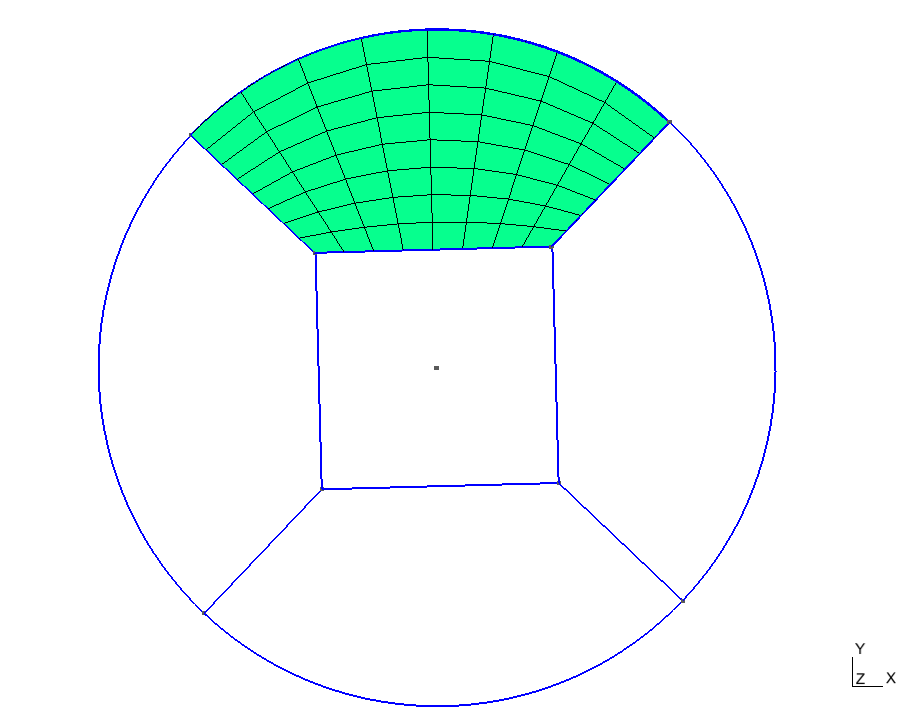
\includegraphics[height=6cm]{figs/lackdisque} 
\par\end{centering}
\caption{\label{fig:macrocell_mesh}Macrocell approach: an example of a mesh
made of five macrocells. Each macrocell is then split into several
subcells. Only the subcells of the top macrocell are represented here
(in green).}
\end{figure}

In \texttt{schnaps} we also defined an \emph{interface} structure
in order to manage data communications between the macrocells. An
interface contains a copy of the data at the Gauss-Lobatto points
that are common to the two neighboring macrocells.

To solve one time step of the DG method, here are the most important
tasks: 
\begin{enumerate}
\item \texttt{Interface\_extraction}: this task simply extracts the values
of $\vw$ coming from the neighboring macrocells to the interface.
In this task, the macrocell buffers are accessed in \texttt{read}
mode and the interface data in \texttt{write} mode. \inmod Of course,
if the interface is a boundary interface, only one side is extracted.\outmod 
\item \texttt{Interface\_fluxes}: this task only computes the numerical
fluxes (\ref{eq:surface_terms}) that are located at the Gauss-Lobatto
points on the interface. The fluxes are then applied to the neighboring
macrocells. In this task, the interface data are accessed in \texttt{read}
mode and the macrocell data in \texttt{read/write} mode. For a better
efficiency, we also assume a \texttt{commute} access to the macrocell
data. In this way the interface fluxes can be assembled in any order,
which can help the StarPU scheduling. 
\item \texttt{Interface\_boundary\_fluxes}: this task computes the boundary
data and only numerical fluxes (\ref{eq:surface_terms}) that are
located at the boundary interface. The fluxes are applied to the neighboring
macrocell. In this task, the interface data are accessed in \texttt{read}
mode and the macrocell data in \texttt{read/write} and \texttt{commute}
mode. 
\item \texttt{Volume\_terms}: this task applies the volumic terms (\ref{eq:volume_terms})
in a given macrocell. The macrocell data are accessed in \texttt{read/write/commute}
mode. 
\item \texttt{Subcell\_fluxes}: this task applies the numerical subcell
fluxes (\ref{eq:surface_terms}) that are internal to a given macrocell.
The macrocell data are accessed in \texttt{read/write/commute} mode.
\item \inmod \texttt{Mass\_matrix}: this task apply the inverse of the
diagonal mass matrix. The macrocell data are accessed in \texttt{read/write}
mode.\outmod 
\end{enumerate}
Additional simple tasks are needed to apply the Runge-Kutta algorithm.
We do not describe them.

The general sequential DG algorithm is then given in Algorithm \ref{alg:DG-algorithm}.
Thanks to StarPU, this algorithm can be submitted in a sequential
way. StarPU then uses the data dependency in order to distribute the
tasks in parallel on the available workers. The wait for task completion
is done at the end of the algorithm and not inside each iteration.
\inmod This is not an essential point for performance but we have
observed in some cases a 15\% gain compared to an algorithm with a
synchronization point at the end of each time iteration. Let us also
observe that this synchronization strategy assumes that the time step
is known at the beginning of the computations. This is not always
possible especially when solving non-linear systems.\outmod 

\begin{algorithm}
\ForAll{interfaces}{
\tcp{task (1)}
Extract interface (copy the data from the neighboring macrocells to the interface)\;
\eIf{the interface is a boundary interface}
{\tcp{task (3)}
compute the boundary fluxes (Equation~\ref{eq:surface_terms}) and apply them to the neighboring macrocell\;}
{\tcp{task (2)}
the interface is an internal one. Compute the numerical fluxes (Equation~\ref{eq:surface_terms}) and apply them to the two neighboring macrocells\;}
}
\ForEach{macrocell}{
\tcp{task (5)}
Compute and apply the numerical fluxes (Equation~\ref{eq:surface_terms}) between the subcells \;
\tcp{task (4)}
Compute the volume terms (Equation~\ref{eq:volume_terms}) inside the subcells\;
\tcp{task(6)}
Apply the inverse of the mass matrix (Equation~\ref{eq:mass_matrix}) inside the subcells \;
}
% for all interface:
% Extract interface (copy the data from the neighboring macrocells to the interface). This is task (1).
% If the interface is a boundary interface, compute the boundary fluxes () and apply them to the neighboring macrocell (task (3));
% Else the interface is an internal one. Compute the numerical fluxes () and apply them to the two neighboring macrocells (task (2)).
% End for
% Then, for each macrocell:
% Compute and apply the numerical fluxes () between the subcells (task (5)).
% Compute the volume terms () inside the subcells (task (4)).
% Apply the inverse of the mass matrix () inside the subcells (task(6)).
% End for

\caption{\label{alg:DG-algorithm}\inmod Sequential DG algorithm. The parallelism
is automatically detected by StarPU, thanks to the data dependency.\outmod }
\end{algorithm}

In the next section we give more details about the implementation
of the OpenCL codelets.

\section{\label{sec:Hybrid-C/OpenCL-codelets}Hybrid C/OpenCL codelets}

In order to attain better performance, we programmed an OpenCL version
of the previously described codelets. \textcolor{black}{The CPU workers
will continue to use the kernels implemented in C, while the GPU workers
will use the ones in OpenCL.} \inmod When computing on GPUs, it is
generally advised to care about memory access in order to improve
coalescence \cite{helluy:hal-00759135}. \outmod The values of $\v w$
at the Gauss-Lobatto points are stored into what we call a \emph{field}
structure. A field is attached to a macrocell. A given component of
$\v w$ in a field is located thanks to its subcell index \texttt{ic},
a Gauss-Lobatto index \texttt{ig} in the cell, and a component index
\texttt{iw}. If the macrocell is cut into $n_{r}$ subcells in each
direction, if the polynomial order is $d$ and for a system of $m$
conservation laws, these indices have the following bounds 
\[
0\leq\mathtt{ic}<n_{r}^{3},\quad0\leq\mathtt{ig}<(d+1)^{3},\quad0\leq\mathtt{iw}<m.
\]

The values of $\v w$ in a given field are stored into a memory buffer
\texttt{wbuf}. In order to test several memory arrangements, the index
in the buffer is computed by a function \texttt{varindex(ic,ig,iw)}
that we can easily change. For instance, we can consider the following
formula, in which the electromagnetic components at a given Gauss-Lobatto
point are grouped in memory 
\begin{equation}
\mathtt{varindex(ic,ig,iw)=iw+}m\mathtt{*(ig+}(d+1)^{3}\mathtt{*ic)},\label{eq:by_comp}
\end{equation}
or this formula 
\begin{equation}
\mathtt{varindex(ic,ig,iw)=ig+}(d+1)^{3}\mathtt{*(iw+}m\mathtt{*ic)},\label{eq:by_gauss_point}
\end{equation}
in which the electromagnetic components are separated in memory. \inmod A
few years ago, we could observe large differences in performance between
the two strategies. Here, we have not observed significant differences,
maybe because the cache memory of the GPUs used in this work (NVIDIA
GTX 1050 or NVIDIA P100) is now larger.\outmod 

We have programmed an OpenCL codelet for each task described in Section
\ref{subsec:Macrocell-approach}. The most time-consuming kernels
are: (i) the kernel associated to the computations of the volume terms
(\ref{eq:volume_terms}) inside the macrocells, \emph{volume} kernel,
and (ii) the kernel that computes the subcell fluxes, the \emph{surface}
kernel. Boundary and interface terms generally involve fewer computations.

A natural distribution of the workload is to associate one subcell
to each OpenCL work-group and the computations at a Gauss point to
a work-item. With this natural distribution, formula (\ref{eq:by_gauss_point})
ensures optimal coalescent memory access in the volume kernel, but
the access is no more optimal in the surface kernel, because neighboring
Gauss points on the subcell interfaces are not necessarily close in
memory. Therefore, we prefer considering formula (\ref{eq:by_comp}).

\section{Numerical results}

In this section, we present some practical experiments that we realized
with \texttt{schnaps}. The first experiment deals with the efficiency
of the StarPU C99 codelets on a multicore CPU. The second experiment
deals with the efficiency of the OpenCL codelets. Then we test the
code in a CPU/GPU configuration.

We approximate by the DG algorithm an exact plane wave solution of
the Maxwell equations 
\[
\v E=c\left(\begin{array}{c}
-v\\
u\\
0
\end{array}\right),\quad\v H=c\left(\begin{array}{c}
0\\
0\\
1
\end{array}\right),\quad\lambda=0,\quad\mu=0.
\]
with $c=-\cos(\pi/2(ux^{1}+vx^{2}-t))$ and $(u,v)=(\cos(\pi/4),\sin(\pi/4)).$

\inmod For validation purpose, we have first checked the numerical
order of the method. For this, we consider a cubic domain
\[
\Omega=]0,1[^{3}.
\]
We apply the exact solution at the boundary $\partial\Omega$ and
in $\Omega$ at the initial time $t=0$. We perform numerical simulations
for a given final time $T$. We vary the order $d$ of the polynomial
in the DG method and the mesh refinement. We compare the error of
the method in the discrete $L^{2}$ norm (computed with Gauss-Lobatto
numerical integration) at that final time $t=T.$ In a log scale,
we obtain the curves of Figure \ref{fig:num_conv}. As other authors
(see, for instance, \cite{hesthaven2004discontinuous,hindenlang2012explicit}),
we observe that the order of convergence is between $d$ and $d+1$.
With Gauss-Legendre numerical integration we would have obtained more
precise results \cite{kopriva2010quadrature}.

\begin{figure}

\begin{centering}
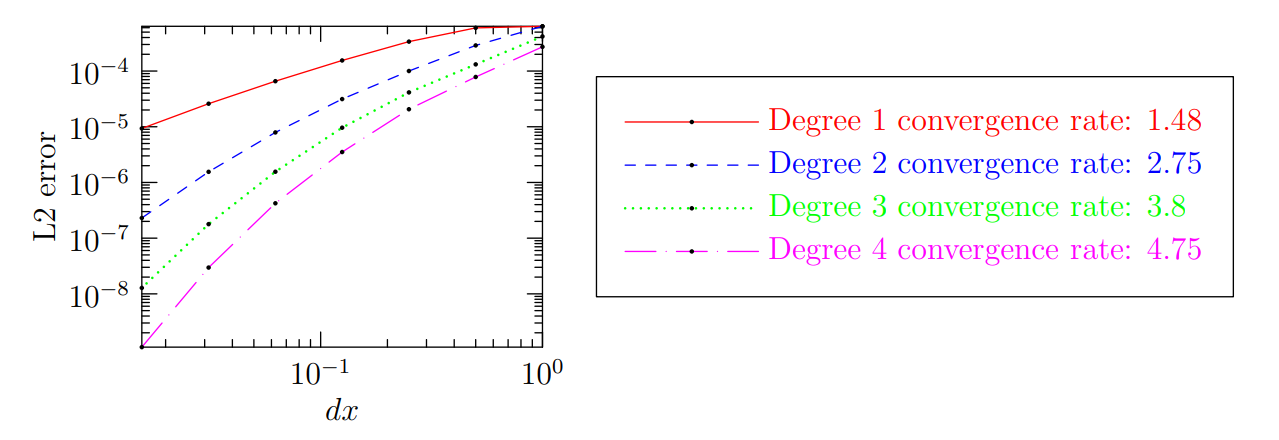
\includegraphics[width=0.8\textwidth]{figs/conv_rate}\caption{Numerical convergence rates for the DG method with Gauss-Lobatto numerical
integration. Plane wave case in a cube.\label{fig:num_conv}}
\par\end{centering}
\end{figure}

\outmod We consider the propagation of the previous electromagnetic
plane wave into a torus-shaped domain $\Omega$ represented on Figure
\ref{fig:Computational-domain}. In the DG solver, we consider only
third order polynomials: $d=3$. The domain is split into $M=400$
macrocells. The macrocells are split into $n_{r}$ subcells in each
direction. The number of degrees of freedom is thus 
\[
n_{\text{d.o.f.}}=Mm(d+1)^{3}n_{r}^{3},\quad M=400,\quad m=8,\quad d=3.
\]

StarPU will have to take decisions on how to distribute efficiently
the tasks on the available accelerators. We have performed our experiments
on two different computers. The first configuration ``PC'' correspond
to a standard desktop personal computer. The second configuration
``WS'' is made of a more powerful two-CPU workstation. The technical
details are listed in Table \ref{tab:config_specs}.

\begin{table}
\centering{}\resizebox{0.9\linewidth}{!}{%
\begin{tabular}{|c|c|c|c|c|c|}
\hline 
config.  & CPU  & \# cores  & mem. CPU  & GPU  & mem. GPU\tabularnewline
\hline 
\hline 
``PC''  & {\small{}{}AMD FX-8320E 3.2 GHz}  & 8  & 8 GB  & {\small{}{}NVIDIA GTX 1050 Ti}  & 4 GB\tabularnewline
\hline 
``WS''  & {\small{}{}Intel Xeon E5-2683 v4 2.1GHz}  & 2$\times$16 & 256 GB  & {\small{}{}NVIDIA P100}  & 16 GB\tabularnewline
\hline 
\end{tabular}}\caption{\label{tab:config_specs}Configurations of the computers used for
the tests.}
\end{table}


\subsection{Multicore CPU tests}

In the first test, we only activate the C99 codelets, and thus the
GPU is not activated. We also vary the number of computing CPU cores
from 2 to 7 for the ``PC'' configuration and from 2 to 31 for the
``WS'' configuration. One CPU core is anyway reserved for the main
StarPU thread.

We perform a fixed number of $n_{t}$ iterations of the RK2 algorithm.
We assume that the number of elementary computing operations increases
as $O(n_{r}^{3}).$ Ideally, with infinitely fast operations at interfaces,
and with \inmod $n_{\text{cpu}}$\outmod  identical CPU cores, the
computations time would behave like 
\begin{equation}
T\sim Cn_{t}\frac{n_{r}^{3}}{n_{\text{cpu}}}\label{eq:ideal_time}
\end{equation}
where $C$ is fixed constant, depending on the hardware. In our benchmark
the \emph{efficiency} is the ratio of the measured execution time
over this ideal time. Normally it should be smaller than one (because
of communications). If it is close to one, the algorithm is very efficient.
In Table \ref{tab:bench_pc_cpu} and \ref{tab:bench_ws_cpu}, we observe
an excellent efficiency of the StarPU task distribution on the CPU
cores even on a NUMA (Non Uniform Memory Access) computer with two
CPUs connected to different memory zones.

\begin{table}
\centering{}%
\begin{tabular}{|c|c|c|c|c|}
\hline 
$n_{r}$  & $n_{\text{cpu}}$  & Time (s)  & Ideal time  & Efficiency\tabularnewline
\hline 
\hline 
4  & 2  & 704  & 704  & 1\tabularnewline
\hline 
4  & 4  & 365  & 352  & 0.96\tabularnewline
\hline 
4  & 7  & 209  & 201  & 0.96\tabularnewline
\hline 
6  & 7  & 689  & 679  & 0.99\tabularnewline
\hline 
8  & 4  & 2902  & 2816  & 0.97\tabularnewline
\hline 
8  & 7  & 1650  & 1609  & 0.98\tabularnewline
\hline 
\end{tabular}\caption{\label{tab:bench_pc_cpu}Efficiency (with two threads as reference)
of the CPU codelets for the ``PC'' configuration with the \texttt{dmdar}
scheduler.}
\end{table}

\begin{table}
\inmod \centering{}%
\begin{tabular}{|c|c|c|c|c|}
\hline 
$n_{r}$  & $n_{\text{cpu}}$  & Time (s)  & Ideal time  & Efficiency\tabularnewline
\hline 
\hline 
4  & 1 & 646 & 646  & 1\tabularnewline
\hline 
4 & 2 & 331 & 323 & 0.97\tabularnewline
\hline 
4 & 4 & 183.4 & 161.5 & 0.88\tabularnewline
\hline 
4 & 8 & 95.1 & 80.7 & 0.85\tabularnewline
\hline 
4 & 16 & 48 & 40.3 & 0.84\tabularnewline
\hline 
4 & 30 & 26  & 21.5 & 0.82\tabularnewline
\hline 
6 & 1  & 2172.1 & 2172.1 & 1\tabularnewline
\hline 
6 & 2 & 1106.7 & 1086 & 0.98\tabularnewline
\hline 
6 & 4 & 612.2 & 543 & 0.88\tabularnewline
\hline 
6 & 8 & 317 & 271.5 & 0.85\tabularnewline
\hline 
6 & 16 & 159 & 135.8 & 0.85\tabularnewline
\hline 
6 & 30 & 85.2 & 72.4 & 0.84\tabularnewline
\hline 
8  & 1 & 5139.4  & 5139.4 & 1\tabularnewline
\hline 
8 & 2 & 2613 & 2569.7 & 0.98\tabularnewline
\hline 
8 & 4 & 1446.6 & 1284.9 & 0.88\tabularnewline
\hline 
8 & 8 & 749.1 & 642.4 & 0.85\tabularnewline
\hline 
8 & 16 & 375.2 & 321.2 & 0.85\tabularnewline
\hline 
8  & 30  & 200.6 & 171.3  & 0.85\tabularnewline
\hline 
\end{tabular}\caption{\label{tab:bench_ws_cpu}Efficiency of the CPU codelets for the ``WS''
configuration with the \texttt{laheteroprio} scheduler.}
\outmod 
\end{table}


\subsection{OpenCL codelets}

\begin{sloppypar} In this section, we compare the efficiency of the
CPU/C99 and GPU/OpenCL codelets on the two configurations ``PC''
and ``WS''. We first perform a CPU-only computation with all the
cores activated (7 for the ``PC'' platform and 31 for the ``WS''
platform) and a GPU-only computation. The results are given in Table
\ref{tab:bench_cpu_gpu}. We observe that the OpenCL codelets are
faster than the CPU codelets. The highest efficiency is achieved for
the finer meshes ($n_{r}=8$ \textcolor{black}{$t_{\text{CPU+2xGPU}}$}).
\end{sloppypar}

\begin{table}
\inmod \centering{}%
\begin{tabular}{|>{\centering}p{0.4cm}|>{\centering}p{1cm}|>{\centering}p{1.1cm}|>{\centering}p{1cm}|>{\centering}p{1cm}|>{\centering}p{1cm}|>{\centering}p{1cm}|>{\centering}p{1cm}|>{\centering}p{1cm}|>{\centering}p{1.15cm}|>{\centering}p{1.5cm}|}
\hline 
$n_{r}$  & config.  & CPU & GPU & 2xGPU & CPU/ GPU & CPU/ 2xGPU & CPU+ GPU & CPU+ 2xGPU & CPU/ {\tiny{}CPU+GPU} & CPU/ {\tiny{}CPU+2xGPU}\tabularnewline
\hline 
\hline 
4  & PC  & 209 s  & 73 s  & - & 2.86  & - & 32 s & - & 6.53 & -\tabularnewline
\hline 
6  & PC  & 689 s & 86 s & - & 8.01  & - & 64 s & - & 10.77 & -\tabularnewline
\hline 
8  & PC  & 1650 s & 171 s  & - & 9.65 & - & 130 s & - & 12.69 & -\tabularnewline
\hline 
4 & WS  & 26 s  & 23.2 s & 18.1 s & 1.12 & 1.43 & 10.7 s & 8.9 s & 2.4 & 2.9\tabularnewline
\hline 
6 & WS & 85.2 s & 26.1 s & 20.3 s & 3.2 & 4.19 & 16.7 s & 11 s & 5.1 & 7.8\tabularnewline
\hline 
8  & WS  & 200.6 s & 29.8 s & 24.3 s & 6.7 & 8.23 & 29.8 s & 18.1 s & 6.7 & 11\tabularnewline
\hline 
\end{tabular}\caption{\label{tab:bench_cpu_gpu}Efficiency of the CPU/GPU implementation.
All timings are given in seconds. All ratio are dimensionless. This
table shows that StarPU is always able to harness an increase of hybrid
computing capacities.}
\outmod 
\end{table}

\begin{figure}
\begin{centering}
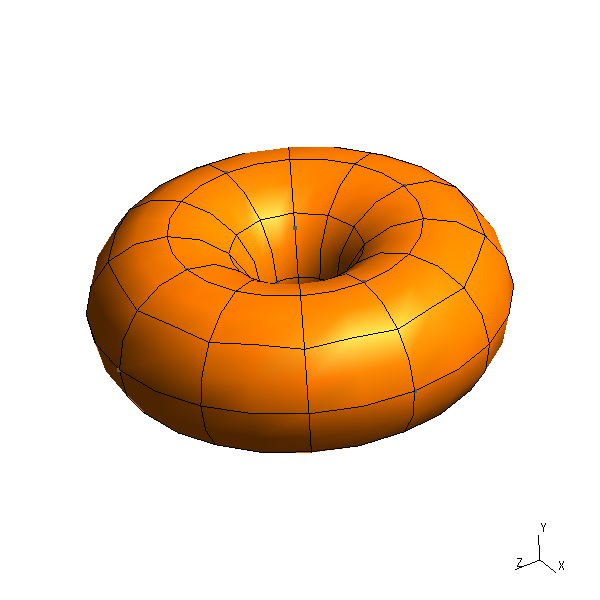
\includegraphics[clip,width=6cm]{figs/test_torus} 
\par\end{centering}
\caption{\label{fig:Computational-domain}Computational domain $\Omega$. Only
the macrocells of the mesh are visible. The represented mesh contains
240 macrocells (poloidal refinement set to $n_{pol}=3$ and toroidal
refinement set to $n_{tor}=3$. In the numerical experiments, we take
$n_{pol}=3$ and $n_{tor}=5$, which leads to a mesh of 400 macrocells).
Each macrocell is then cut regularly into the three directions. }
\end{figure}


\subsection{Hybrid CPU/GPU computations}

\begin{sloppypar} Now that we are equipped with verified OpenCL codelets
we can try to run the code with StarPU in order to see if it is able
to distribute the tasks efficiently on the available accelerators.
\end{sloppypar}

One difficulty is to manage the data transfers efficiently between
the accelerators. Several scheduling strategies are available in StarPU.
With the \texttt{eager} scheduler, the tasks are distributed in the
order of submission to the inactive device, without taking into account
the cost of memory transfers. This strategy is obviously not optimal.

It is better to choose another scheduler. For the ``PC'' configuration,
we use the \texttt{dmda} scheduler provided by StarPU and we use the
\texttt{LAHeteroprio} scheduler (\cite{10.7717/peerj-cs.190}) for
the ``WS'' configuration. With the \texttt{LAHeteroprio} scheduler,
the different types of tasks are grouped into buckets and the processing
unit pick tasks following an order based on their type, which is CPU
or GPU in our case, and the location of the data. The idea is to reduce
the memory transfer and to promote the consumption of the tasks by
the processing units that are more efficient. Therefore, we configure
\texttt{LAHeteroprio} by sorting the different operations by arithmetic
cost and we specify that the CPU workers should follow this order,
while the GPU workers do the opposite: the GPU workers first try to
pick tasks with high workloads. Additionally, we ensure that GPU workers
privilegiate data locality over priorities. Therefore, the distribution
of the tasks on the available CPU cores and GPU is done dynamically
by the scheduler.

The results are given in the last two columns of Table \ref{tab:bench_cpu_gpu}.
We observe that in \textcolor{black}{most }situations, StarPU is able
to get an additional gain from the CPU cores, even if the GPU codelets
are faster. \textcolor{black}{The fact that for $n_{r}=8$ we have
the same execution time with one CPU and one GPU($t_{\text{CPU+GPU}}$),
or with only one GPU ($t_{\text{GPU}}$) is an illustration of the
cost of moving data. More precisely, consider an execution where all
the tasks are on the GPU. Using the CPU would mean moving data on
it, way and back, and thus can imply an overhead, even if the CPU
could be faster for some tasks.}

\section{Conclusion}

We have proposed an optimized implementation of the Discontinuous
Galerkin method on hybrid computer made of several GPUs and multicore
CPUs. In order to manage the heterogeneous architecture easily and
efficiently, we rely on OpenCL for the GPU computations and on the
StarPU runtime for distributing the computational tasks on the available
devices.

OpenCL programming becomes much easier because the task dependency
is computed by StarPU. We only had to concentrate on the optimization
of the individual OpenCL kernels and not on data distribution or memory
transfers. We first tested the efficiency of our OpenCL kernels. We
verified that the macrocell approach and cache prefetching strategy,
while not optimal, give good results.

In addition, with a good choice of scheduler, and for heavy computations,
we have shown that StarPU is able to overlap computations and memory
transfer in a quite efficient way. It is also able to use the available
CPU codelets to achieve even higher acceleration.

\bibliographystyle{plain}
\bibliography{schnaps_opencl2017.bib}

\end{document}
